
La primer ampliación ha sido la incorporación de documentación del programa. Aunque el
término de ampliación no es del todo correcto, puesto que en el proyecto original el autor
elaboró una extensa documentación, esta quedó inaccesible.

\bigskip
La documentación fue realizada en formato .HLP, un formato de ayuda de Windows que quedó
en desuso en Windows Vista. Y esta documentación era realmente interesante, pues no sólo
contenía datos sobre la palicación, sino que incluía consejos para el desarrollo de 
aplicaciones para las distintas máquinas y además explicaba el funcionamiento de las máquinas.

\bigskip
Para recuperar esta documentación se ha utilizado una herramientas de extracción denominada
Help Decompiler. Esta herramienta de línea de comandos procesa los ficheros de ayuda de
Windows .HLP y genera un fichero de texto enriquecido con la documentación y en una carpeta
externa el contenido multimedia que incluye la misma.

\bigskip
Para poder llevar a cabo la tarea de la documentación de forma paralela se consideró que lo mejor era
hacer un proyecto aparte. Resultaba evidente que la documentación de una aplicación web debía de estar en la
web. 

\bigskip
Tras barajar algunas opciones, se optó por mover la documentación a un formato mantenible como 
es markdown. Y partiendo de esto se utilizó un generador de contenido estático basado en NodeJS (Hexo)
para convertir este markdown en web. Se desarrollo un tema simple y personalizado para la ayuda y se 
añadió la capacidad de cambiar entre inglés y español.

\bigskip
Este es el estado actual de la aplicación de la documentación.

\begin{figure}[!th]
\begin{center}
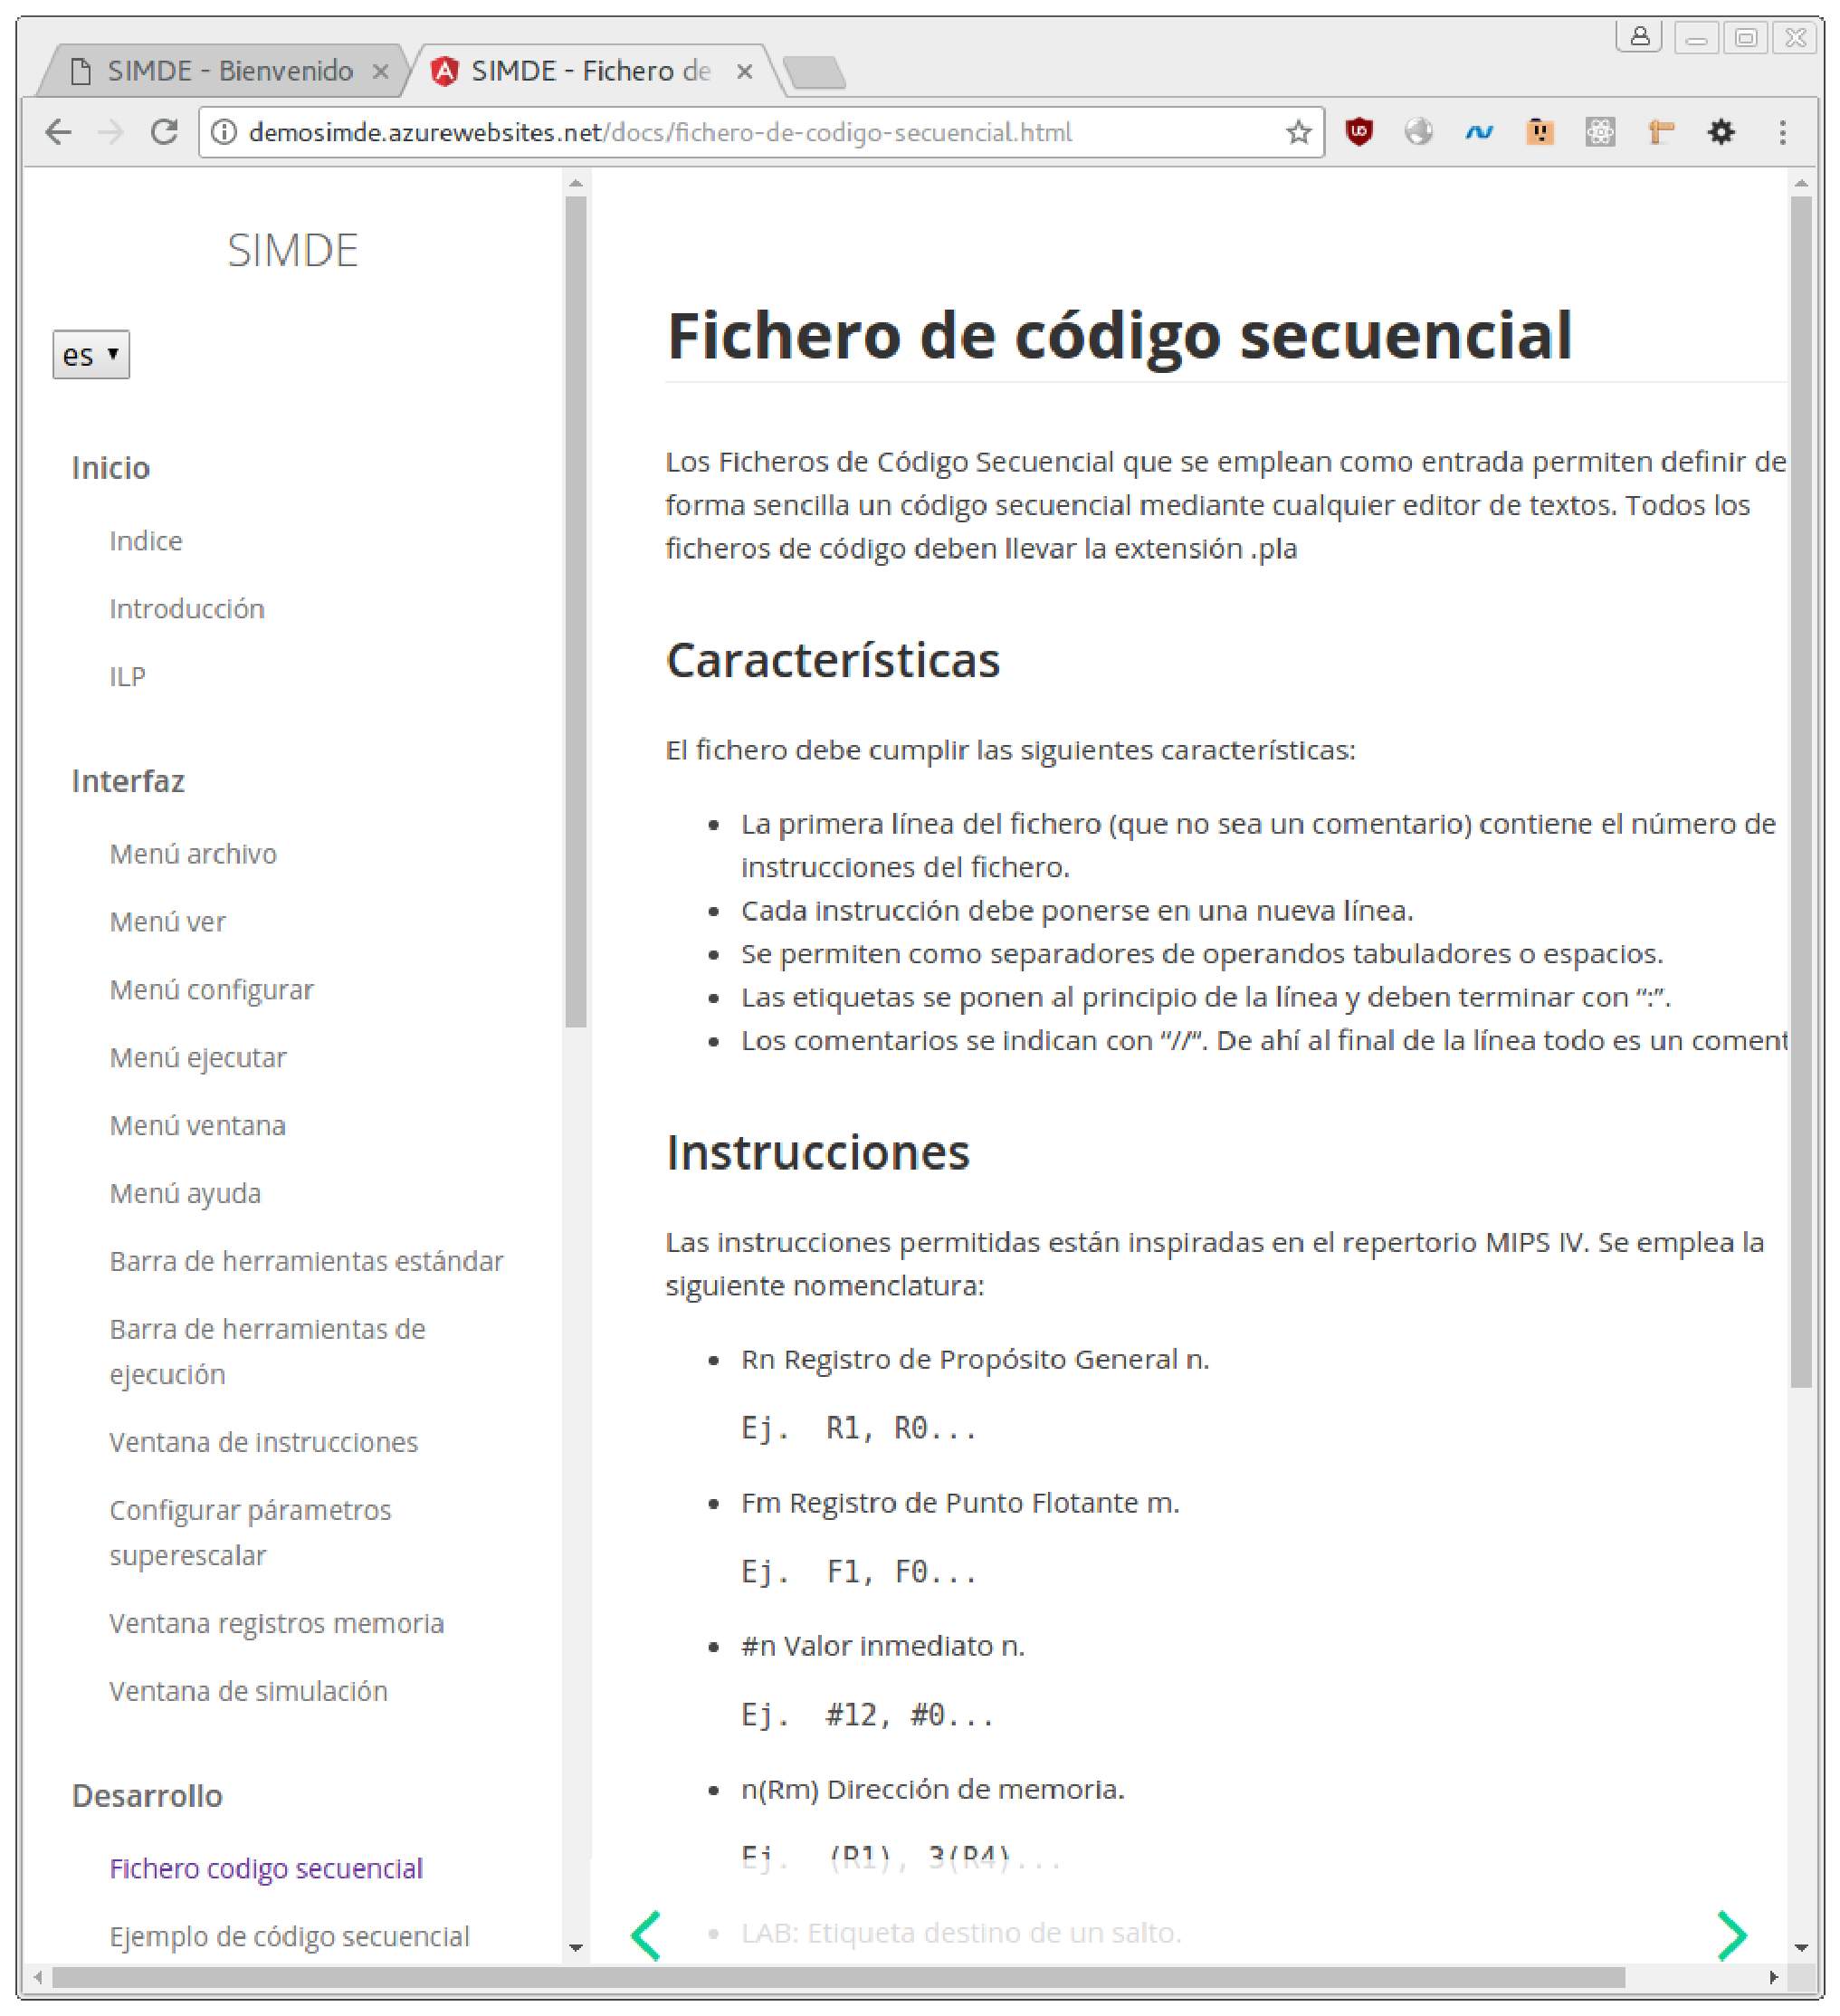
\includegraphics[width=0.5\textwidth]{images/cap5/nueva-documentacion.eps}
\caption{Nueva version de la documentacion}
\label{fig:Nueva version de la documentacion}
\end{center}
\end{figure}

\bigskip
Se puede acceder a ella desde el menú \textit{Ayuda - Documentación} en la nueva aplicación del SIMDE.